\documentclass[12pt]{report}
\usepackage[utf8]{inputenc}
\usepackage[english]{babel}
\usepackage{titlesec}
\usepackage{comment}
\usepackage{listings, xcolor}
\usepackage{amsmath}
\usepackage{amsfonts}

\usepackage[
backend=biber,
style=alphabetic,
sorting=ynt
]{biblatex}
\addbibresource{literatur.bib}

\usepackage{graphicx}
\graphicspath{{images/}}   % where are the images

\author{Eugenio\ Gallea (s241876) \\ Stefano\ Roagna (s241845)}
\title{"It's tracking"\ Term Report \\ Distributed Programming 2}
\date{February 2018}

\titleformat{\chapter}
  {\normalfont\LARGE\bfseries}{\thechapter}{1em}{}
\titlespacing*{\chapter}{0pt}{3.5ex plus 1ex minus .2ex}{2.3ex plus .2ex}

\lstset{
tabsize = 4, %% Sets tab space width.
showstringspaces = false, %% Prevents space marking in strings, string is defined as the text that is generally printed directly to the console.
numbers = left, %% Displays line numbers on the left.
commentstyle = \color{green}, %% Sets comment color.
keywordstyle = \color{blue}, %% Sets  keyword color.
stringstyle = \color{red}, %% Sets  string color.
rulecolor = \color{black}, %% Sets frame color to avoid being affected by text color.
basicstyle = \small \ttfamily , %% Sets listing font and size.
breaklines = true, %% Enables line breaking.
numberstyle = \tiny,
}

\renewcommand{\lstlistingname}{Snippet}
\renewcommand{\lstlistlistingname}{List of \lstlistingname s}

%%%----------------------------------------------------------
\begin{document}
%%%----------------------------------------------------------
\maketitle
\tableofcontents
%%%----------------------------------------------------------
\chapter{Summary}\label{Chap:Summary}
The aim of this project has been the one to design a \textbf{RESTful web service} able to \underline{track} the precence of vehicles in a area with \textbf{restricted access} and, based on this information, choose if \underline{guarantee or reject} the access to other vehicles. If the \textit{access is granted}, the system, has to provide the client application, of the newly-entered vehicle, with a \textit{suggested path to follow}. Otherwise, the vehicle is just \textit{rejected by the system} with a message.\\
In order to be able to \textbf{track} the vehicle, the client application has to sent \underline{periodically} (every time a new place is entered) information about the current position. At any point in time, the vehicle can decide \underline{not to follow} the suggested path, in this case the system has to be able to provide the client with a \textit{new route, if possible}.\\

%%%----------------------------------------------------------
\chapter{Architecture}\label{Chap:Architecture}
\begin{figure}[!htb]
   \centering
   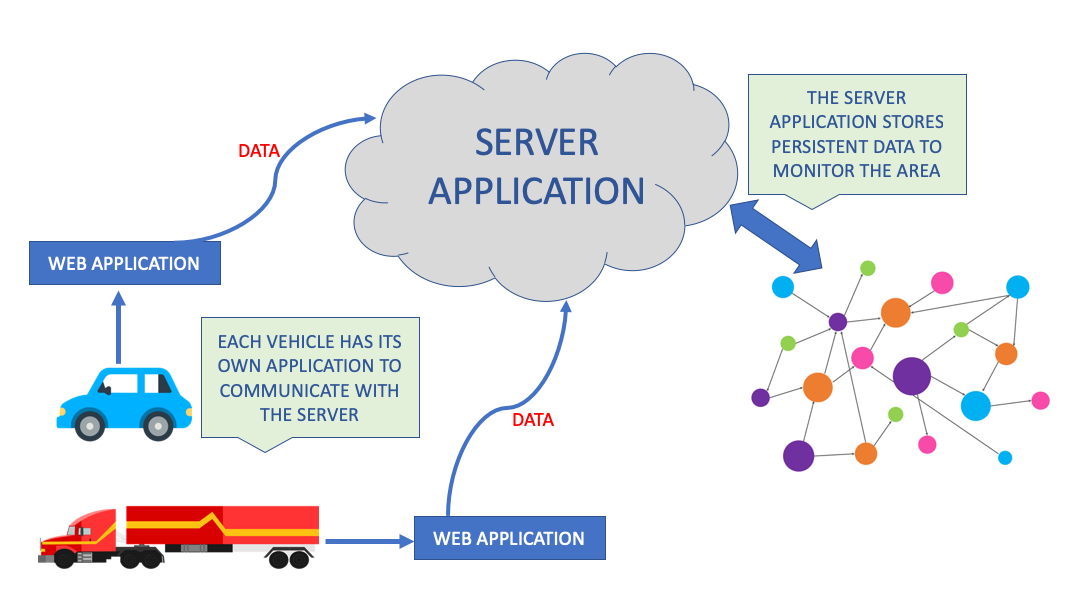
\includegraphics[width=\textwidth]{architecture.png}
   \caption{Architecture of the system.}\label{Fig:ArchNoImpl}
\end{figure}
The system consists of three principal components:
\begin{itemize}
  \item Server: this component is responsible for the validation of data, supervision of the system and interaction with the database
    to store persistent data;
  \item Client: this component consist of an application, located on the vehicle, that communicates with the server and provide it with information about the vehicle (e.g. position, entry and exit time);
  \item Database: where are stored data about the current state of the area, i.e. actual capacity of places, position of vehicles and
  average times spent in each place.
\end{itemize}

%%%----------------------------------------------------------
\chapter{Implementation}\label{Chap:Impl}
\section{Used technologies}
\begin{figure}[!htb]
   \centering
   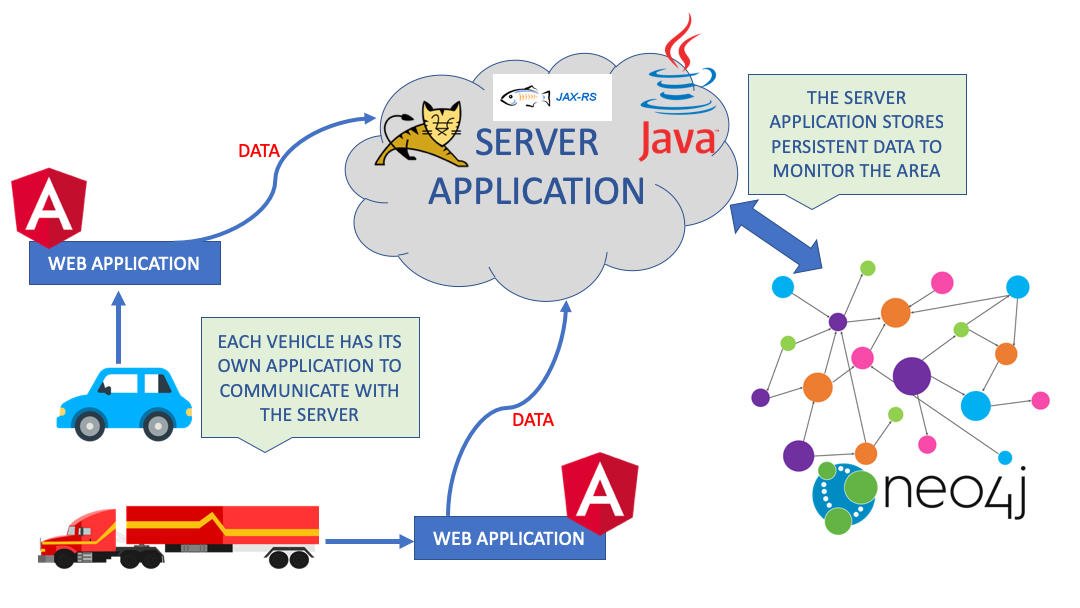
\includegraphics[width=\textwidth]{architecture_impl.png}
   \caption{Architecture of the system with which technologies have been used for each component.}\label{Fig:ArchImpl}
\end{figure}
In figure \ref{Fig:ArchImpl} are presented the various components of the system along with the technologies used to achieve the objectives of each one. In particular:
\begin{itemize}
  \item for the \underline{server} application have been used various technologies:
    \begin{enumerate}
      \item \textbf{Apache Tomcat} is an open source software that implements a \textit{web server}, i.e. it manages the handling of Java Servlets, JSP. It is used to deploy web applications developed in Java \parencite{tomcat}.
      \item \textbf{JAX-RS} has been used as a framework to develop REST application, given the used language has been \textbf{Java}.
    \end{enumerate}
  \item for the \underline{database} component it has been decided to use \textbf{Neo4j} as storage for persistent data. Since what we are operating on (a map of places) can be modeled as connection between nodes, Neo4j, as a graph database, came in handy. Also it allowed to specify the type of relations between different nodes in the database as discussed in chapter \ref{Chap:Neo4j}.
  \item the \underline{client} has been developed in \textbf{Angular}, a platform created to build applications with the web. Angular applications are equally used for mobile and desktop.
\end{itemize}

% --------------------------------------------------------------------------

\section{Communication between components}
There are two communication channels in this architecture:
\begin{enumerate}
  \item cleint $\leftrightarrow$ server: the server is able to speak both XML and JSON, but for this particular project has been decided to use mainly JSON;
  \item server $\leftrightarrow$ database: in this case the server uses \textbf{Cypher} query language (specific for Neo4j) in order to run queries in the database. As a result it is obtained a pseudo-json from which it is possible to extract the desired data, asked in the query.
\end{enumerate}

% --------------------------------------------------------------------------

%%%----------------------------------------------------------
\chapter{Data model}\label{Chap:DataModel}
\begin{figure}[!htb]
   \centering
   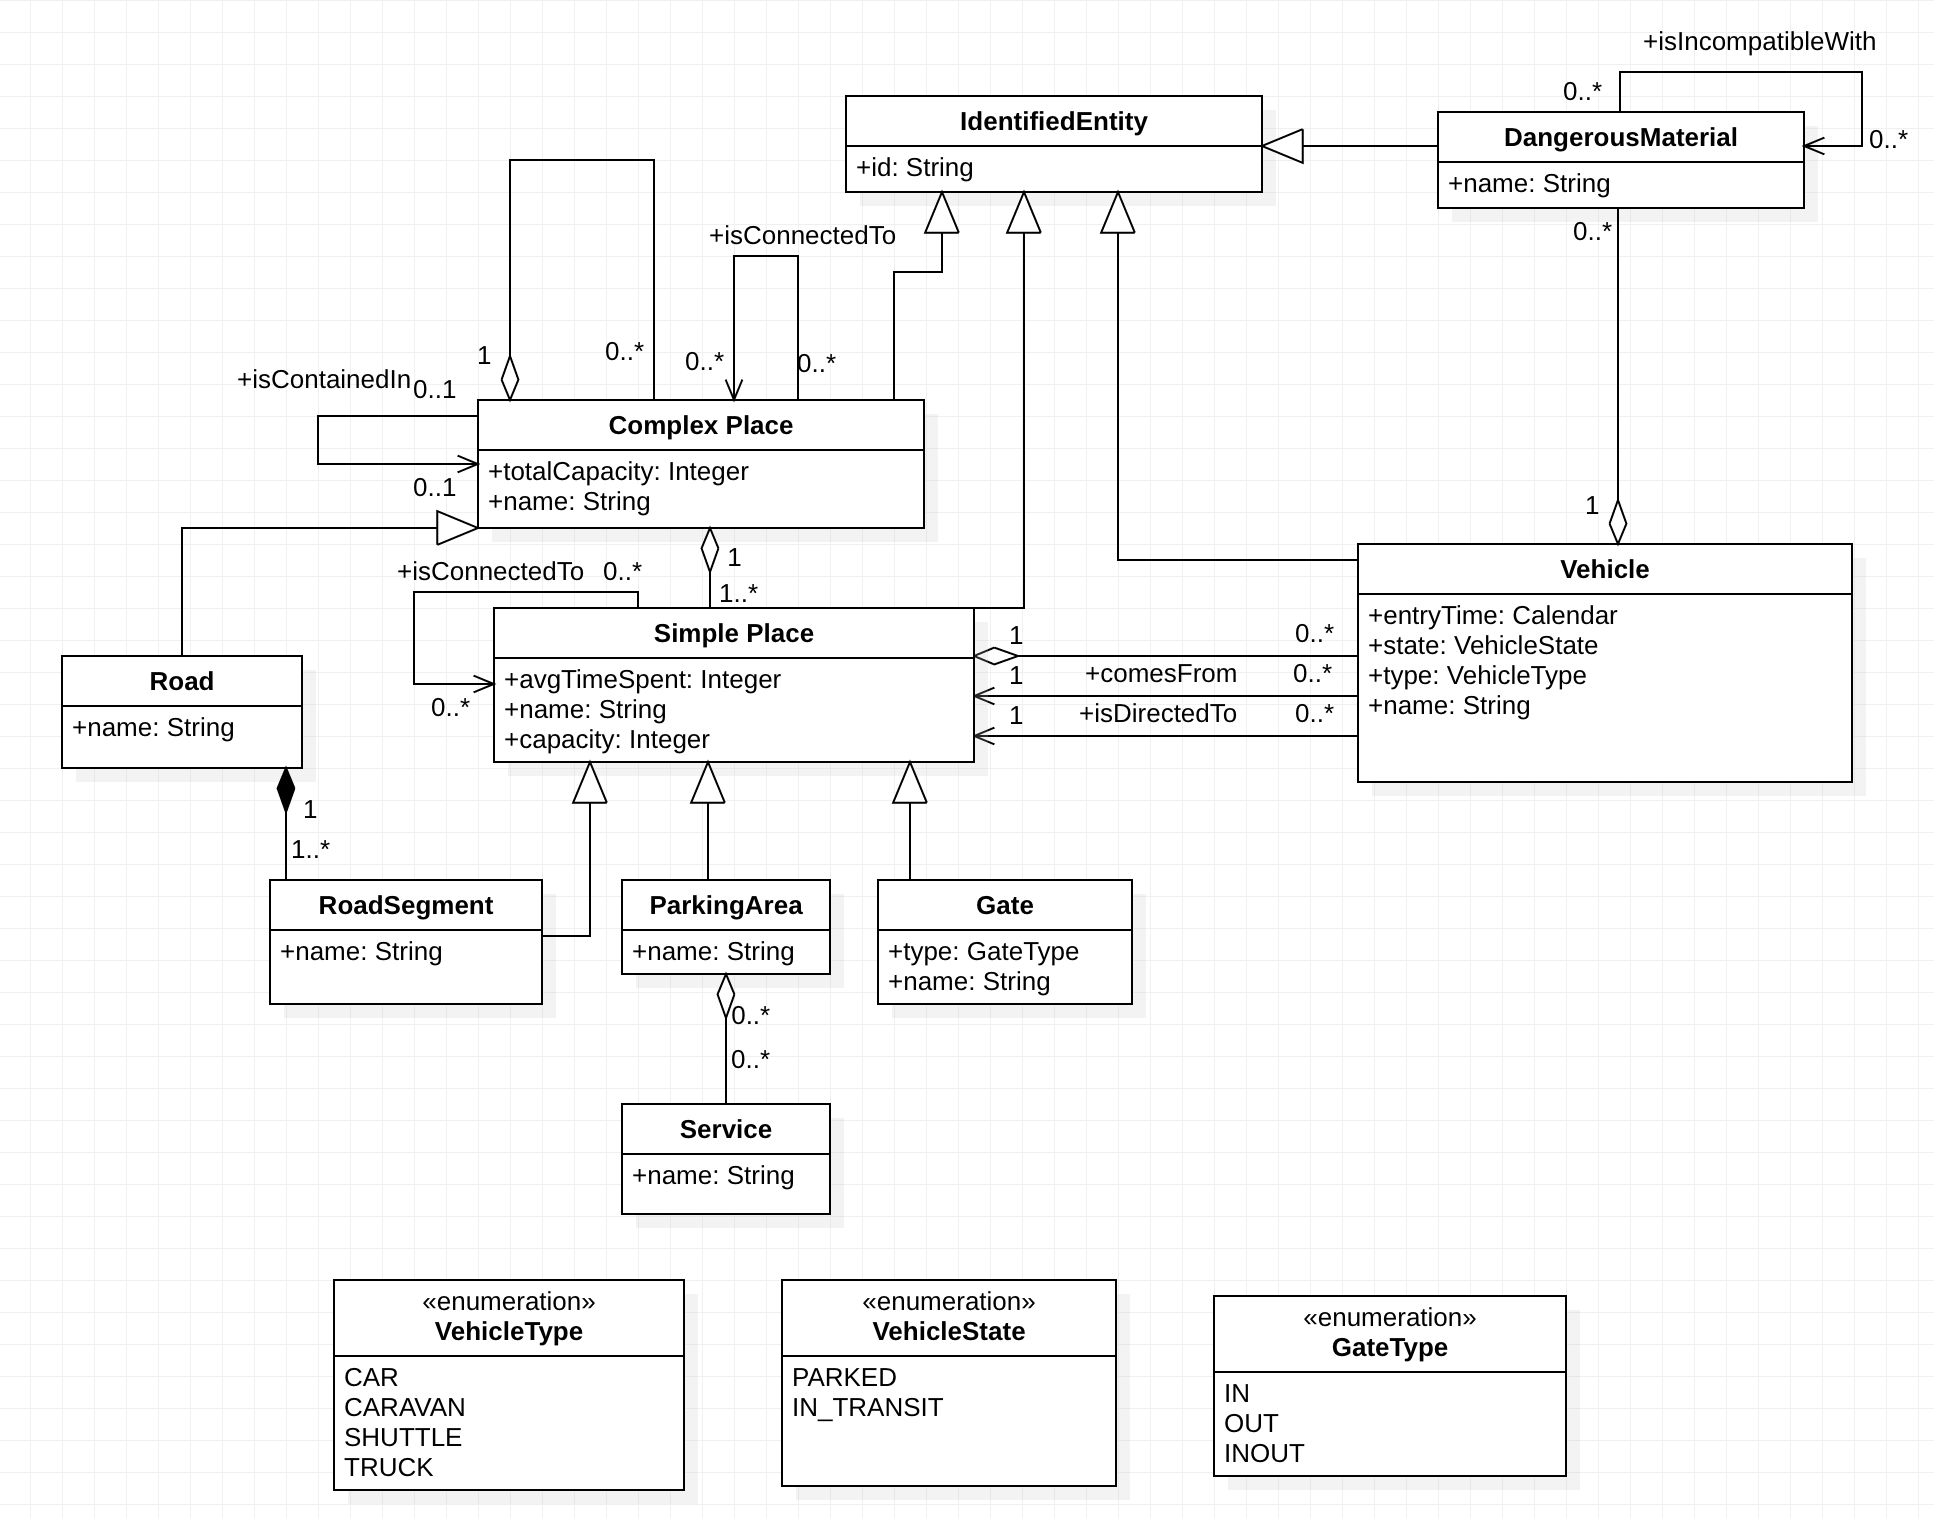
\includegraphics[width=\textwidth]{data_model.png}
   \caption{Data model for the application.}\label{Fig:data_model}
\end{figure}
In figure \ref{Fig:data_model} it is represented the UML model that describes the data handles by the application. Each node of the map can be described as a simple place. Each place has a maximum capacity, that represents the maximum number of vehicle allowed to be in the same time in that place. This property of the places will be exploited as constraint during the evaluation of a path for the entering vehicles. A particularity of this model is the presence of complex places. They have been defined in such way that they can contain a set of simple places or other complex places. For this particular project has been defined only one type of complex place, but if, for future purposes, will be necessary to add other particular complex places, it will be possible to extends the ComplexPlace type.\\
All the information regarding the schema representing the model, are represented in the file \textit{/RNSService/rns/WebContent/WEB-INF/classes/xsd}. The Java classes used in the server application are generated from this file using JAXB.

%%%----------------------------------------------------------
\chapter{Server application}
\section{Application organization}
The server application has been developed and organized according to the multi-tier application paradigm.
\begin{figure}[!htb]
   \centering
   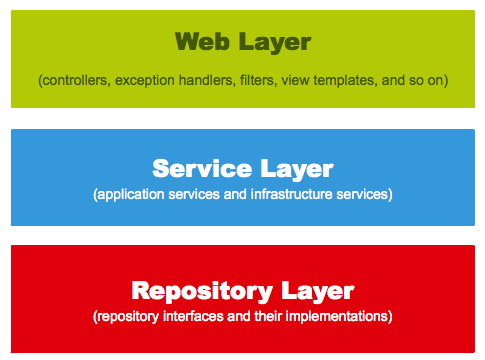
\includegraphics[width=.8\textwidth]{application_layers.png}
   \caption{Subdivision of layers of multi-tier application.}\label{Fig:AppMultiTier}
\end{figure}
Such paradigm is shown in figure \ref{Fig:AppMultiTier} and it states that a web application has to be subdivided in different layers, each one of them with its own responsabilities. It's an approach similar to the \textit{divide et impera} one, where a bigger problem is divided into sub-problems to achieve a solution. Similarly in this case, each layer works indipendently from the other and if they need to communicate, they do it through interfaces connecting them.\\
The organization of the layers in this project has been done this way:
\begin{itemize}
  \item \underline{web (presentation) layer}: all classes whose name ends with \textit{Resource} or \textit{Validator}. They are located in package \textit{it.polito.dp2.rest.rns.resources} and they contain the definition of endpoints or filters used for the REST API to which clients will connect;
  \item \underline{service layer}: this layer is the one responsible of all the business logic of the application and preparation of the information for possible queries to the database. All the logic of the developed application is contained in \textbf{RNSCore.java} class (itself located into \textit{it.polito.dp2.rest.rns.resources} package). To achieve all objectives it is supposed to, it relies on the usage of some utility classes located into package \textit{it.polito.dp2.rest.rns.utility} and to communicate possible errors to the presentation layer it utilizes custom exceptions, contained into package \textit{it.polito.dp2.rest.rns.exceptions};
  \item \underline{repository (database) layer}: this layer has to handle all the interaction with the database. In this case it has been decided to use as a persistent storage Neo4j graph database \cite{neo4j}. This part is discussed more in details in section \ref{Chap:Neo4j}.
\end{itemize}
To test the correctness of the developed application have been used two approaches:
\begin{enumerate}
  \item the development of the client application is a test itself since it simulated a vehicle entering the system and performing random operations as discussed in chapter \ref{Chap:Client};
  \item some basic junit test have been developed and added in package \textit{it.polito.dp2.rest.rns.test.*}. In particular this package is subdivided into other packages \textit{it.polito.dp2.rest.rns.test.tests} and \textit{it.polito.dp2.rest.rns.test.client}: the first contains all the function performing check and assertions on the result of certain operations, the second instead contains functions that instantiate clients to perform requests to specific endpoints.
\end{enumerate}
As they are now, the tests check: if the vehicle that can be added is added correctly and all the information are preserved (POST of a vehicle and GET of the same vehicle); if a client tries to add a vehicle with as entry a place with not enough capacity, receives an error response; if a client tries to add twice a vehicle with the same id, receives an error response.\\
All the endpoint a client can exploit are visible in swagger documentation once the service is up and running. In order to access the full description of it from a browser, it is necessary to follow the link \textit{Swagger documentation} visible when connecting to the homepage of the service at \textit{http://localhost:8080/rns/}.

%%%----------------------------------------------------------
\section{Z3}\label{Z3}
\subsection{What is Z3}
Z3 is a a theorem prover \cite{z3}. It came in handy with our project, since it can be exploited to solve problems that requires the definition of constraints.\\
In particular, Z3, is composed of two components:
\begin{enumerate}
  \item the \textit{OptSMT} module that is used to solve problems regarding the optimization of classical linear arithmetic objective functions (e.g. Knapsack problem \cite{knapsack});
  \item the \textit{MaxSMT} (actually a collection of \underline{MaxSAT} solvers) module that we're most interested in, because it allows the definition of soft contraints in order to evaluate a solution.
\end{enumerate}

% --------------------------------------------------------------------------

\subsection{Setup of Z3 in machine running Ubuntu}
The development enviroment that has been used is \textbf{Ubuntu}. In order to use Z3 library in such operating system, there are a couple of steps one has to follow.
\begin{enumerate}
  \item \underline{download} the prebuilt version of the library from the offical GitHub repository \url{https://github.com/Z3Prover/z3/releases};
  \item once extracted the files, we have to place them in a specific location in which we will command other applications to look for the needed classes;
  \begin{figure}[!htb]
     \centering
     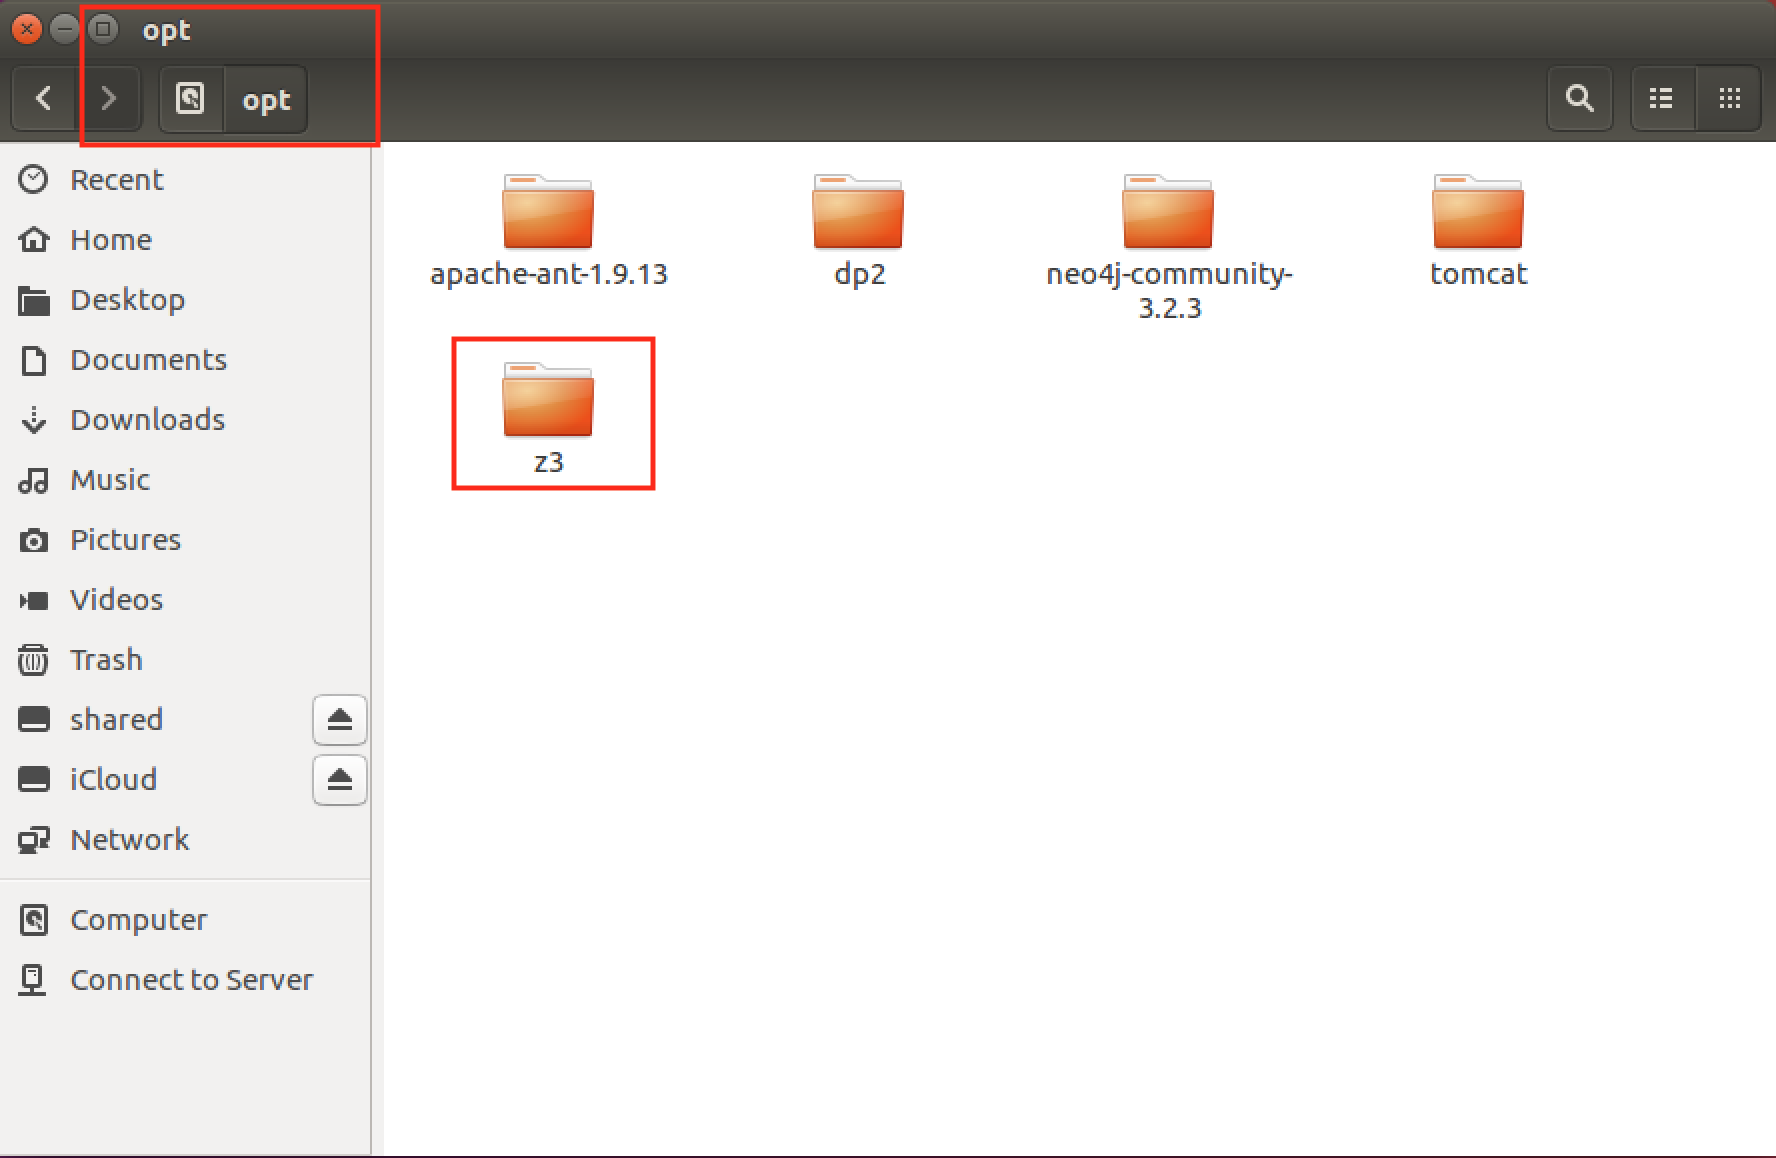
\includegraphics[width=\textwidth]{z3_location.png}
     \caption{Example of where to place Z3 extracted libraries.}\label{Fig:Z3Location}
  \end{figure}
  \item after everything has been placed in the chosen location, we have to \textbf{define} an environment variable which will allow the Java application to know where the Z3 library is located. For Ubuntu such variable is \underline{LD\_LIBRARY\_PATH}. This variable must point to the location of the \underline{bin} folder of the extracted Z3 library;
  \begin{figure}[!htb]
     \centering
     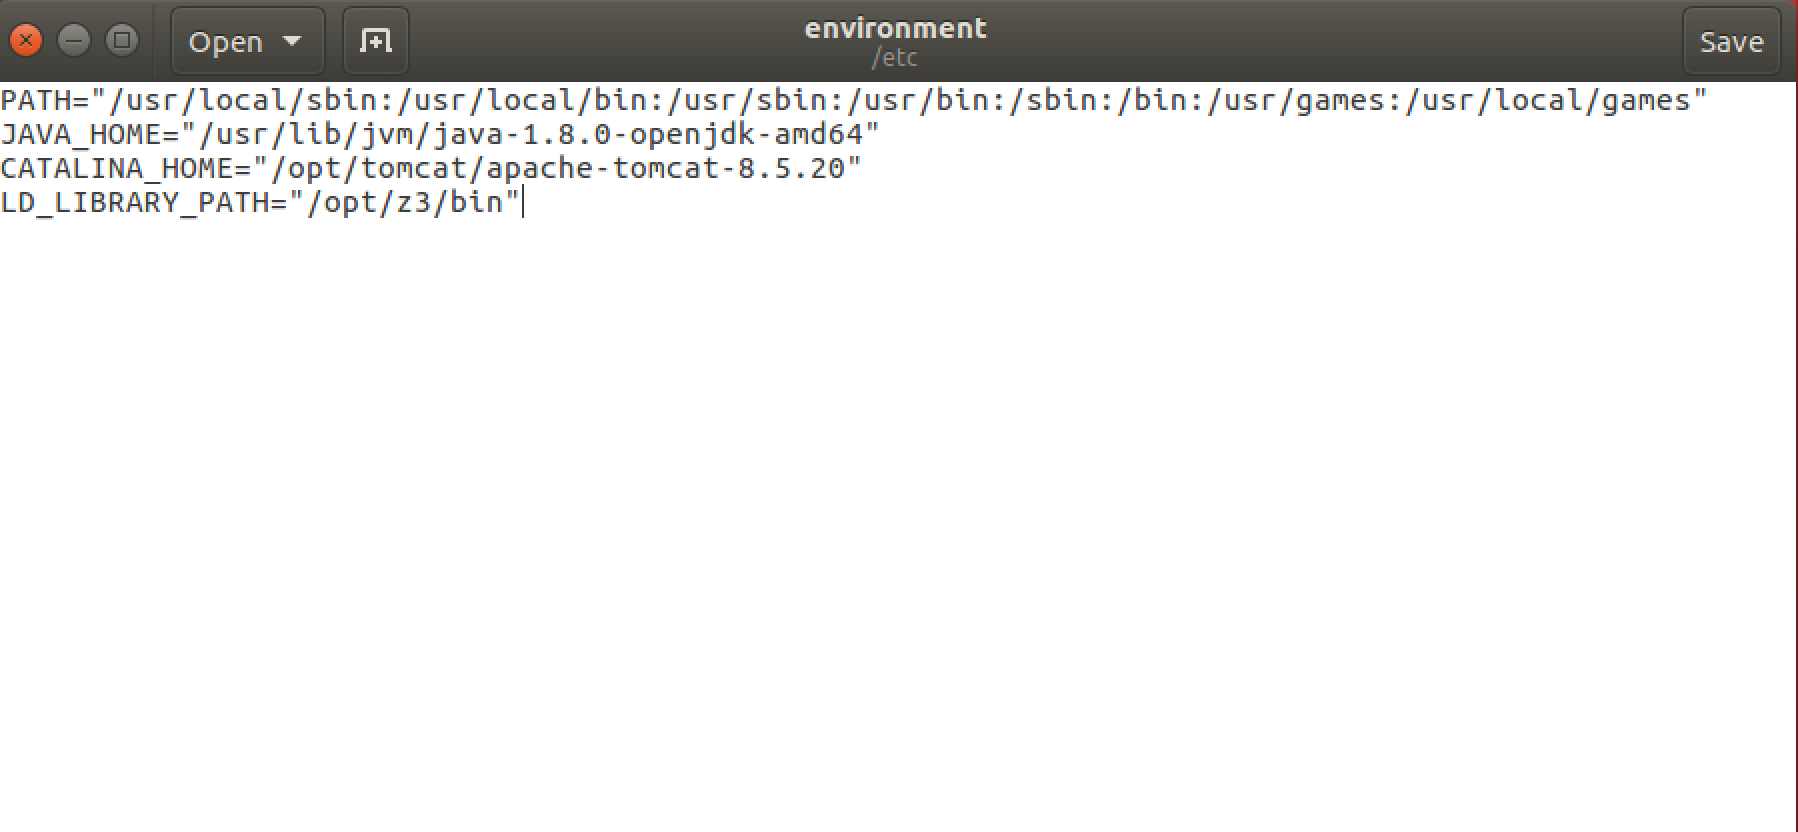
\includegraphics[width=\textwidth]{z3_environment.png}
     \caption{Example of how to define LD\_LIBRARY\_PATH environment variable.}\label{Fig:Z3Environment}
  \end{figure}
  In figure \ref{Fig:Z3Environment} is shown an example of definition of the LD\_LIBRARY\_PATH environment variable. \\
  In this case has been define globally for the whole machine, that means it has been inserted in the file \textit{/etc/environment}, but the same result could have been achieve defining it locally for the used in \textit{/Home/.bashrc} file;
  \item last step, is to add the Z3 .jar file to the build path of our project.
  \begin{figure}[!htb]
     \centering
     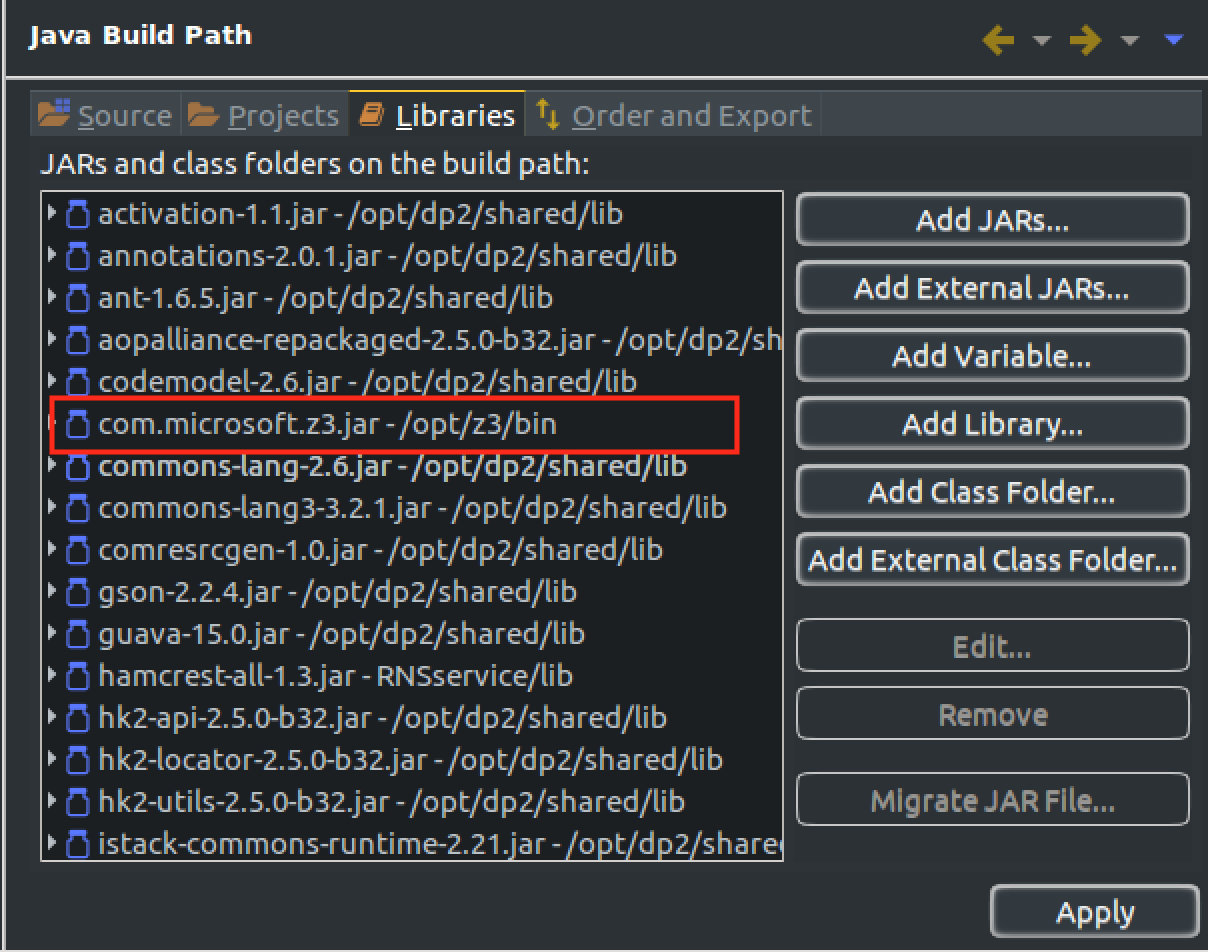
\includegraphics[width=\textwidth]{z3_buildpath.png}
     \caption{Example of how the project build path should look like.}\label{Fig:Z3BuildPath}
  \end{figure}
\end{enumerate}
This is an automatic configuration and Tomcat will load the dynamic libraries in the bin folder by itself. If this is not sufficient, we need to manually put in the WebContent/WEB-INF/lib/jni the Z3 library and point LD\_LIBRARY\_PATH to that folder.\\
Please make sure, in order to use the library in Tomcat, to have correctly set CATALINA\_HOME variable, pointing to Tomcat folder and JAVA\_HOME variable (provided you have installed Java on the machine).

% --------------------------------------------------------------------------

\subsection{Model}
In order to define a model for Z3 to work on, it has been extracted a graph from the actual map, with updated capacities and position of vehicles.\\
The criteria for a node to be selected as a possible node are: 
\begin{itemize}
	\item the node doesn't contain any dangerous material.
	\item the node contains some vehicles carrying dangerous materials, but they are compatible with the one of the new vehicle.\\
\end{itemize}

\subsubsection{Mathematical Model}\label{Subs:MathModel}
The obtained mathematical model is the following.

\paragraph{Objective Function}
\begin{description}
	\item min $\ \sum_{i=1}^{N} y_{i}t_{i}$
\end{description}
\paragraph{Variables}
\begin{description}
	\item \textit{N}: number of nodes of the system
	\item $\ y_{i} \in$ \{0, 1\}: a generic node \textit{i}
	\item $\ c_{i} \geq 0$: the capacity of the node \textit{i}
	\item $\ t_{i} \in \mathbb{N}$: the weight average time spent in the node \textit{i}
	\item $\ y_{ij} \in \{0, 1\}$: a connection from node \textit{i} to node \textit{j} 
\end{description}

\paragraph{Constraints}
\begin{description}
	\item $\ c_{i} \geq y_{i} $
	\item $\ \sum_{i \in N} y_{si} = 1$, where \textit{s} is the origin 
	\item $\ \sum_{i \in N} y_{id} = 1$, where \textit{d} is the destination
	\item $\ \sum_{i,j \in N} y_{ij} - \sum_{i,j \in N} y_{ji} = 0$, where $\ y_{ij}$ are the incoming and $\ y_{ji}$ the outcoming connections 	
\end{description}

\subsubsection{Final result}
The final output of the z3 model consists in a set of boolean variables. If the value is \textbf{true}, that means that the node is to be considered in the path.\\
In the snippet \ref{Snip:Z3Model} there is an example for a path evaluated for a newly entered vehicle.
\begin{lstlisting}[frame = trBL , escapeinside={(*@}{@*)}, caption = Final result that need to be parsed to retrieve ne node ids, captionpos=b, label=Snip:Z3Model]
(define-fun y_a02-01 () Bool true)
(define-fun y_ss02 () Bool true)
(define-fun y_a02-02 () Bool false)
(define-fun y_ss01 () Bool false)
(define-fun y_a01-01 () Bool false)
(define-fun y_a01-02 () Bool true)
(define-fun y_a01-03 () Bool false)
(define-fun y_ss03 () Bool true)
(define-fun y_g05 () Bool true)
(define-fun y_g04 () Bool true)
\end{lstlisting}

% --------------------------------------------------------------------------
\subsection{Example}
In this subsection will be presented an example of how the server will compute the correct path for a new vehicle that wants to enter the system.
\begin{figure}[!htb]
   \centering
   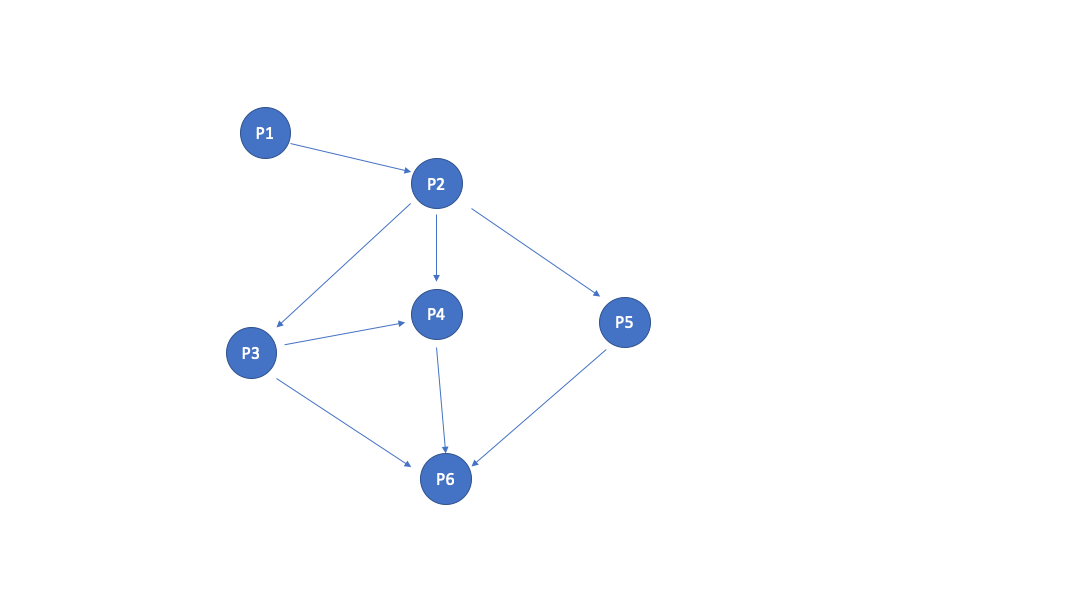
\includegraphics[width=\textwidth]{graph00.png}
   \caption{Example graph.}\label{Fig:Graph00}
\end{figure}
The initial graph that is given Z3 to work on is the one in figure \ref{Fig:Graph00}. Here two assumptions are made:
\begin{enumerate}
  \item node \textbf{P5} contains a vehicle that carries a dangerous material not compatible with the one carried by the new vehicle that wants to enter;
  \item node \textbf{P4} has not enough capacity to accept another vehicle.
\end{enumerate}
The first step that it has to be performed is selecting the origin and destination in the graph (in this case \textbf{P1} and \textbf{P6}) and infer in Z3's optimizer an hard constraint that state that both these nodes has to result \textbf{true} in order to verify the correctness of the solution. The selection of origin node (red) and destination node (green) is shown in fugire \ref{Fig:Graph01}.
\begin{figure}[!htb]
   \centering
   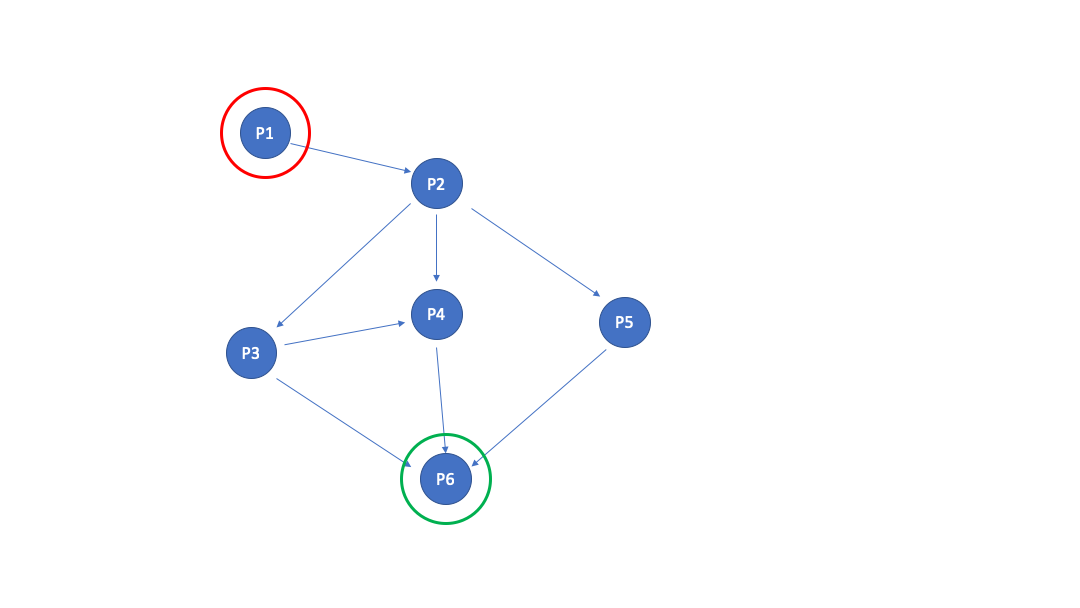
\includegraphics[width=\textwidth]{graph01.png}
   \caption{Selection of origin (red) and destination (green).}\label{Fig:Graph01}
\end{figure}
The next step is pruning from the actual graph, in order to input a correct map to Z3, all the nodes that don't meet the dangerous material constraint. Such constraint states that for a node to be selected it has not to contain any vehicle carrying materials not compatible with the one carried by the vehicle that wants to enter the system. Coherently with assumptions, node \textbf{P5} is pruned out from the graph, since it contains a vehicle with materials not compatible with the new entering (figure \ref{Fig:Graph02}).
\begin{figure}[!htb]
   \centering
   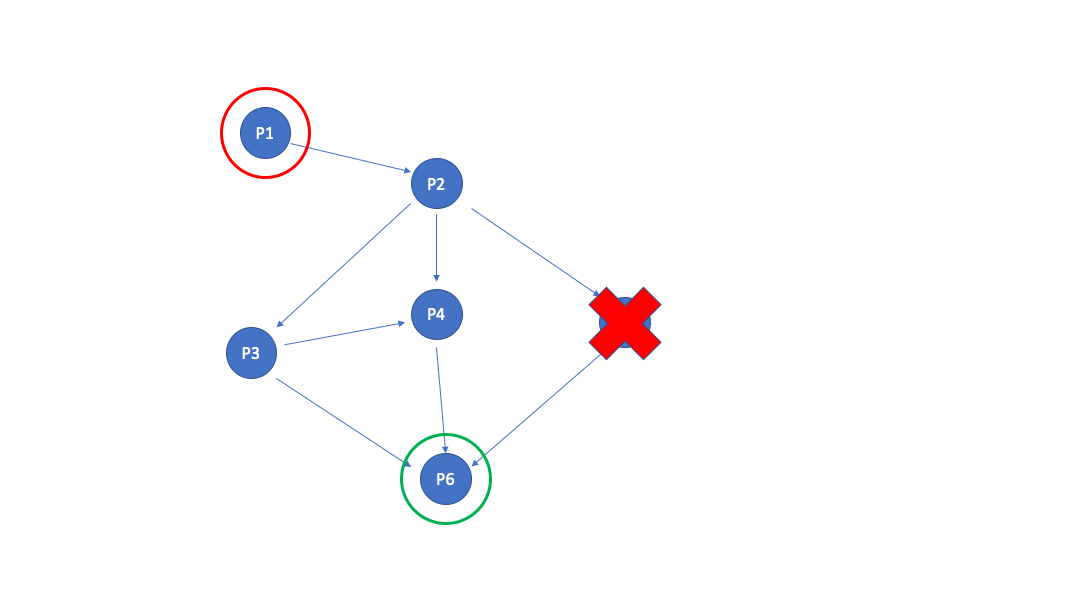
\includegraphics[width=\textwidth]{graph02.png}
   \caption{Pruning of a node due to dangerous materials constraints.}\label{Fig:Graph02}
\end{figure}
Once a correct graph has been retrieve for Z3, the next phase is to define boolean expressions for the optimizer. To achieve that, it is necessary to recur the whole graph in order to explore every node. For each one of them, different expressions has to be defined:
\begin{itemize}
  \item a boolean expression for understanding if a node is considered in the final path, that will result \textbf{true} only if one of its incoming connection's boolean expression is \textbf{true};
  \item a boolean expression for the capacity of the node, that will result to true only if the capacity of the node is greater or equal than 1. If this expression is false, it will invalidate the node as a whole, making it not suitable for the route;
  \item a boolean expression for each one the connection betwee the node and the previous ones. This is not an actual boolean expression, because it is derived from the AND between the two boolean expressions of the nodes at the end of the connection.
\end{itemize}
\begin{figure}[!htb]
   \centering
   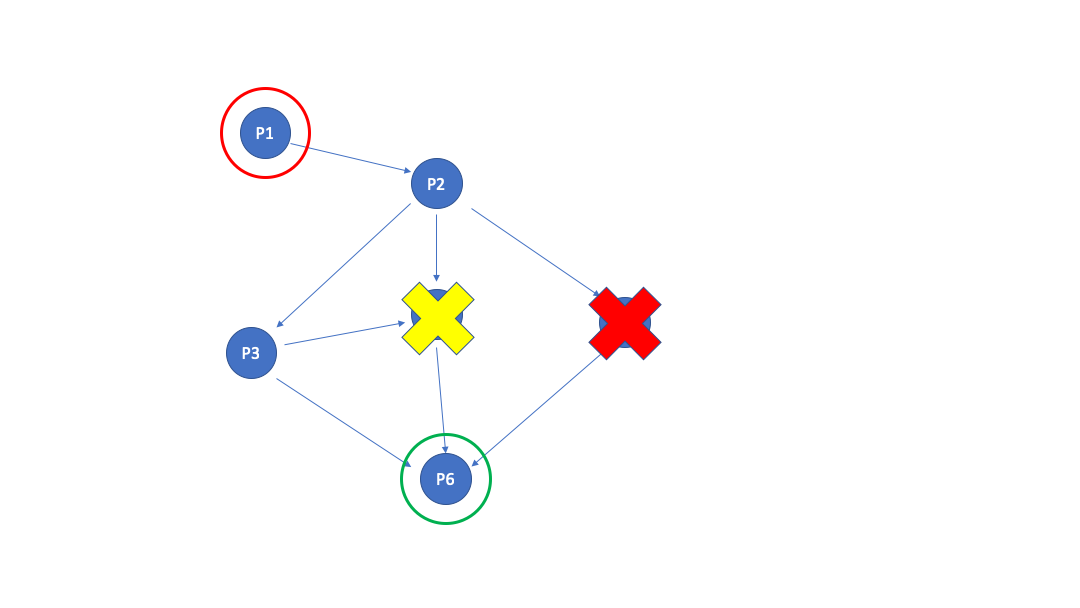
\includegraphics[width=\textwidth]{graph03.png}
   \caption{Pruning of a node due to capacity constraints.}\label{Fig:Graph03}
\end{figure}
Given the definition of such expressions, since the capacity of node \textbf{P4} doesn't meet the requirements as specified above, the corresponding boolean expression of the node is invalidated by the optimized, making it not a suitable node for the evaluation of a path as shown in figure \ref{Fig:Graph03}.
\begin{figure}[!htb]
   \centering
   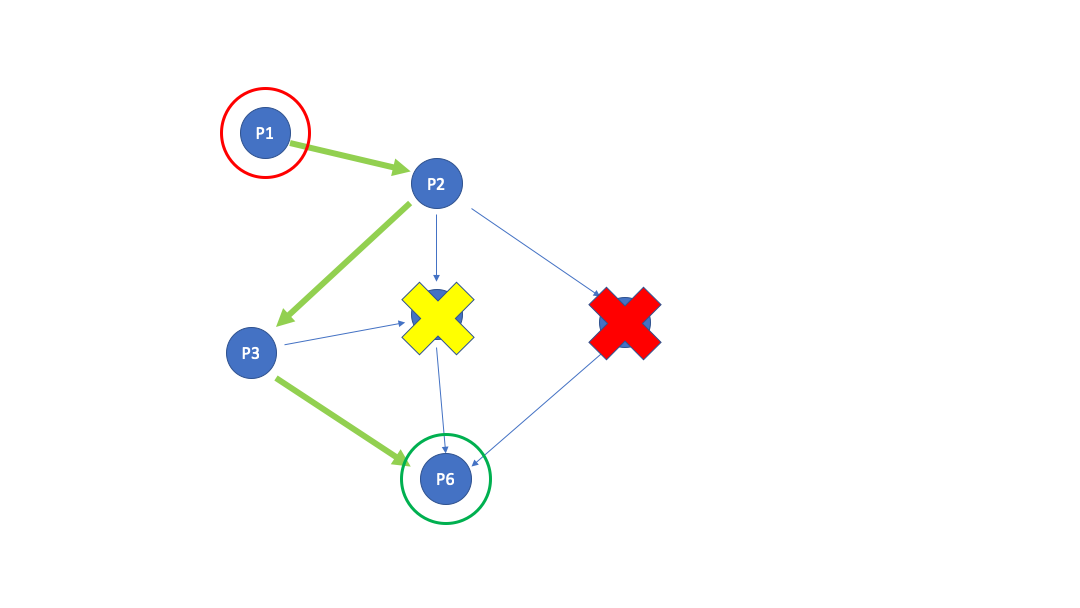
\includegraphics[width=\textwidth]{graph04.png}
   \caption{Evaluation of path from source to destination.}\label{Fig:Graph04}
\end{figure}
The resulting path produced by Z3 is the one show in figure \ref{Fig:Graph04}. In the case multiple paths are present from source to destination, the optimizer will choose the one with the minimum traverse time, using the min time constraint define as subsection \ref{Subs:MathModel} shows.

%%%----------------------------------------------------------
\section{Neo4j} \label{Chap:Neo4j}
As a persistent backend storage, it has been decided to use Neo4j \cite{neo4j}. The main reasons behing this choice are:
\begin{itemize}
  \item ease of use;
  \item a graph database is very handy when working with maps;
  \item neo4j is the leader in the development of graph database frameworks.
\end{itemize}
The developed library for interfacing with the database is located in package \textit{it.polito.dp2.rest.rns.neo4j} and it is based on the usage of Neo4j drivers and Cypher query language, that is one of the two way to go suggested by Neo4j documentation (Cypher and drivers \cite{neo4jcypher} or HTTP rest API \cite{neo4jhttprest}). \\
The package contains two classes:
\begin{enumerate}
  \item class \textbf{Neo4jInteractions.java}: it is used to to start/close a session with the database, execute a query, retrieve the results. It basically offers a set of function to allow the service layer of the server application to store, retrieve, delete and update data;
  \item class \textbf{StatementBuilder.java}: this class is responsbile of providing a set of functions that create statements (a.k.a. queries), to be run in the database through the driver, depending on some parameters that are given.
\end{enumerate}
The access from service layer to database layer is achieved through an object of type \textbf{Neo4jInteractions}. It has been developed using a \textit{singleton} pattern in order to have only one instance of this object for the whole application. Such pattern consists in the definition of a private constructor and a private static instance of an object of the same type of the containing class. This is instance is made accessible through static methods. \\
In the database, each neo4j node corresponds to a place. Since the defined model for the project stated that even connection between places are to be considered places themselves, the relationships between nodes that neo4j offers have been exploited in a different way. What relationships have been used is to describe two things:
\begin{enumerate}
  \item the \underline{type} of relationship existing between the nodes (container, connection, ...);
  \item the \underline{direction} in which is possible to traverse the two nodes. Let's assume there exist two nodes, \textit{node1} and \textit{node2}, that are strongly connected (which means there is a relationship from \textit{node1} to \textit{node2} and one the other way around), a vehicle is able to go either from \textit{node1} to \textit{node2} or from \textit{node2} to \textit{node1}. If there is only one relation, for instance from \textit{node1} to \textit{node2}, the vehicle will only be able to traverse the nodes the same direction the relation is pointing (in this case \textit{node1}$\rightarrow$ \textit{node2}).
\end{enumerate}
\begin{figure}[!htb]
   \centering
   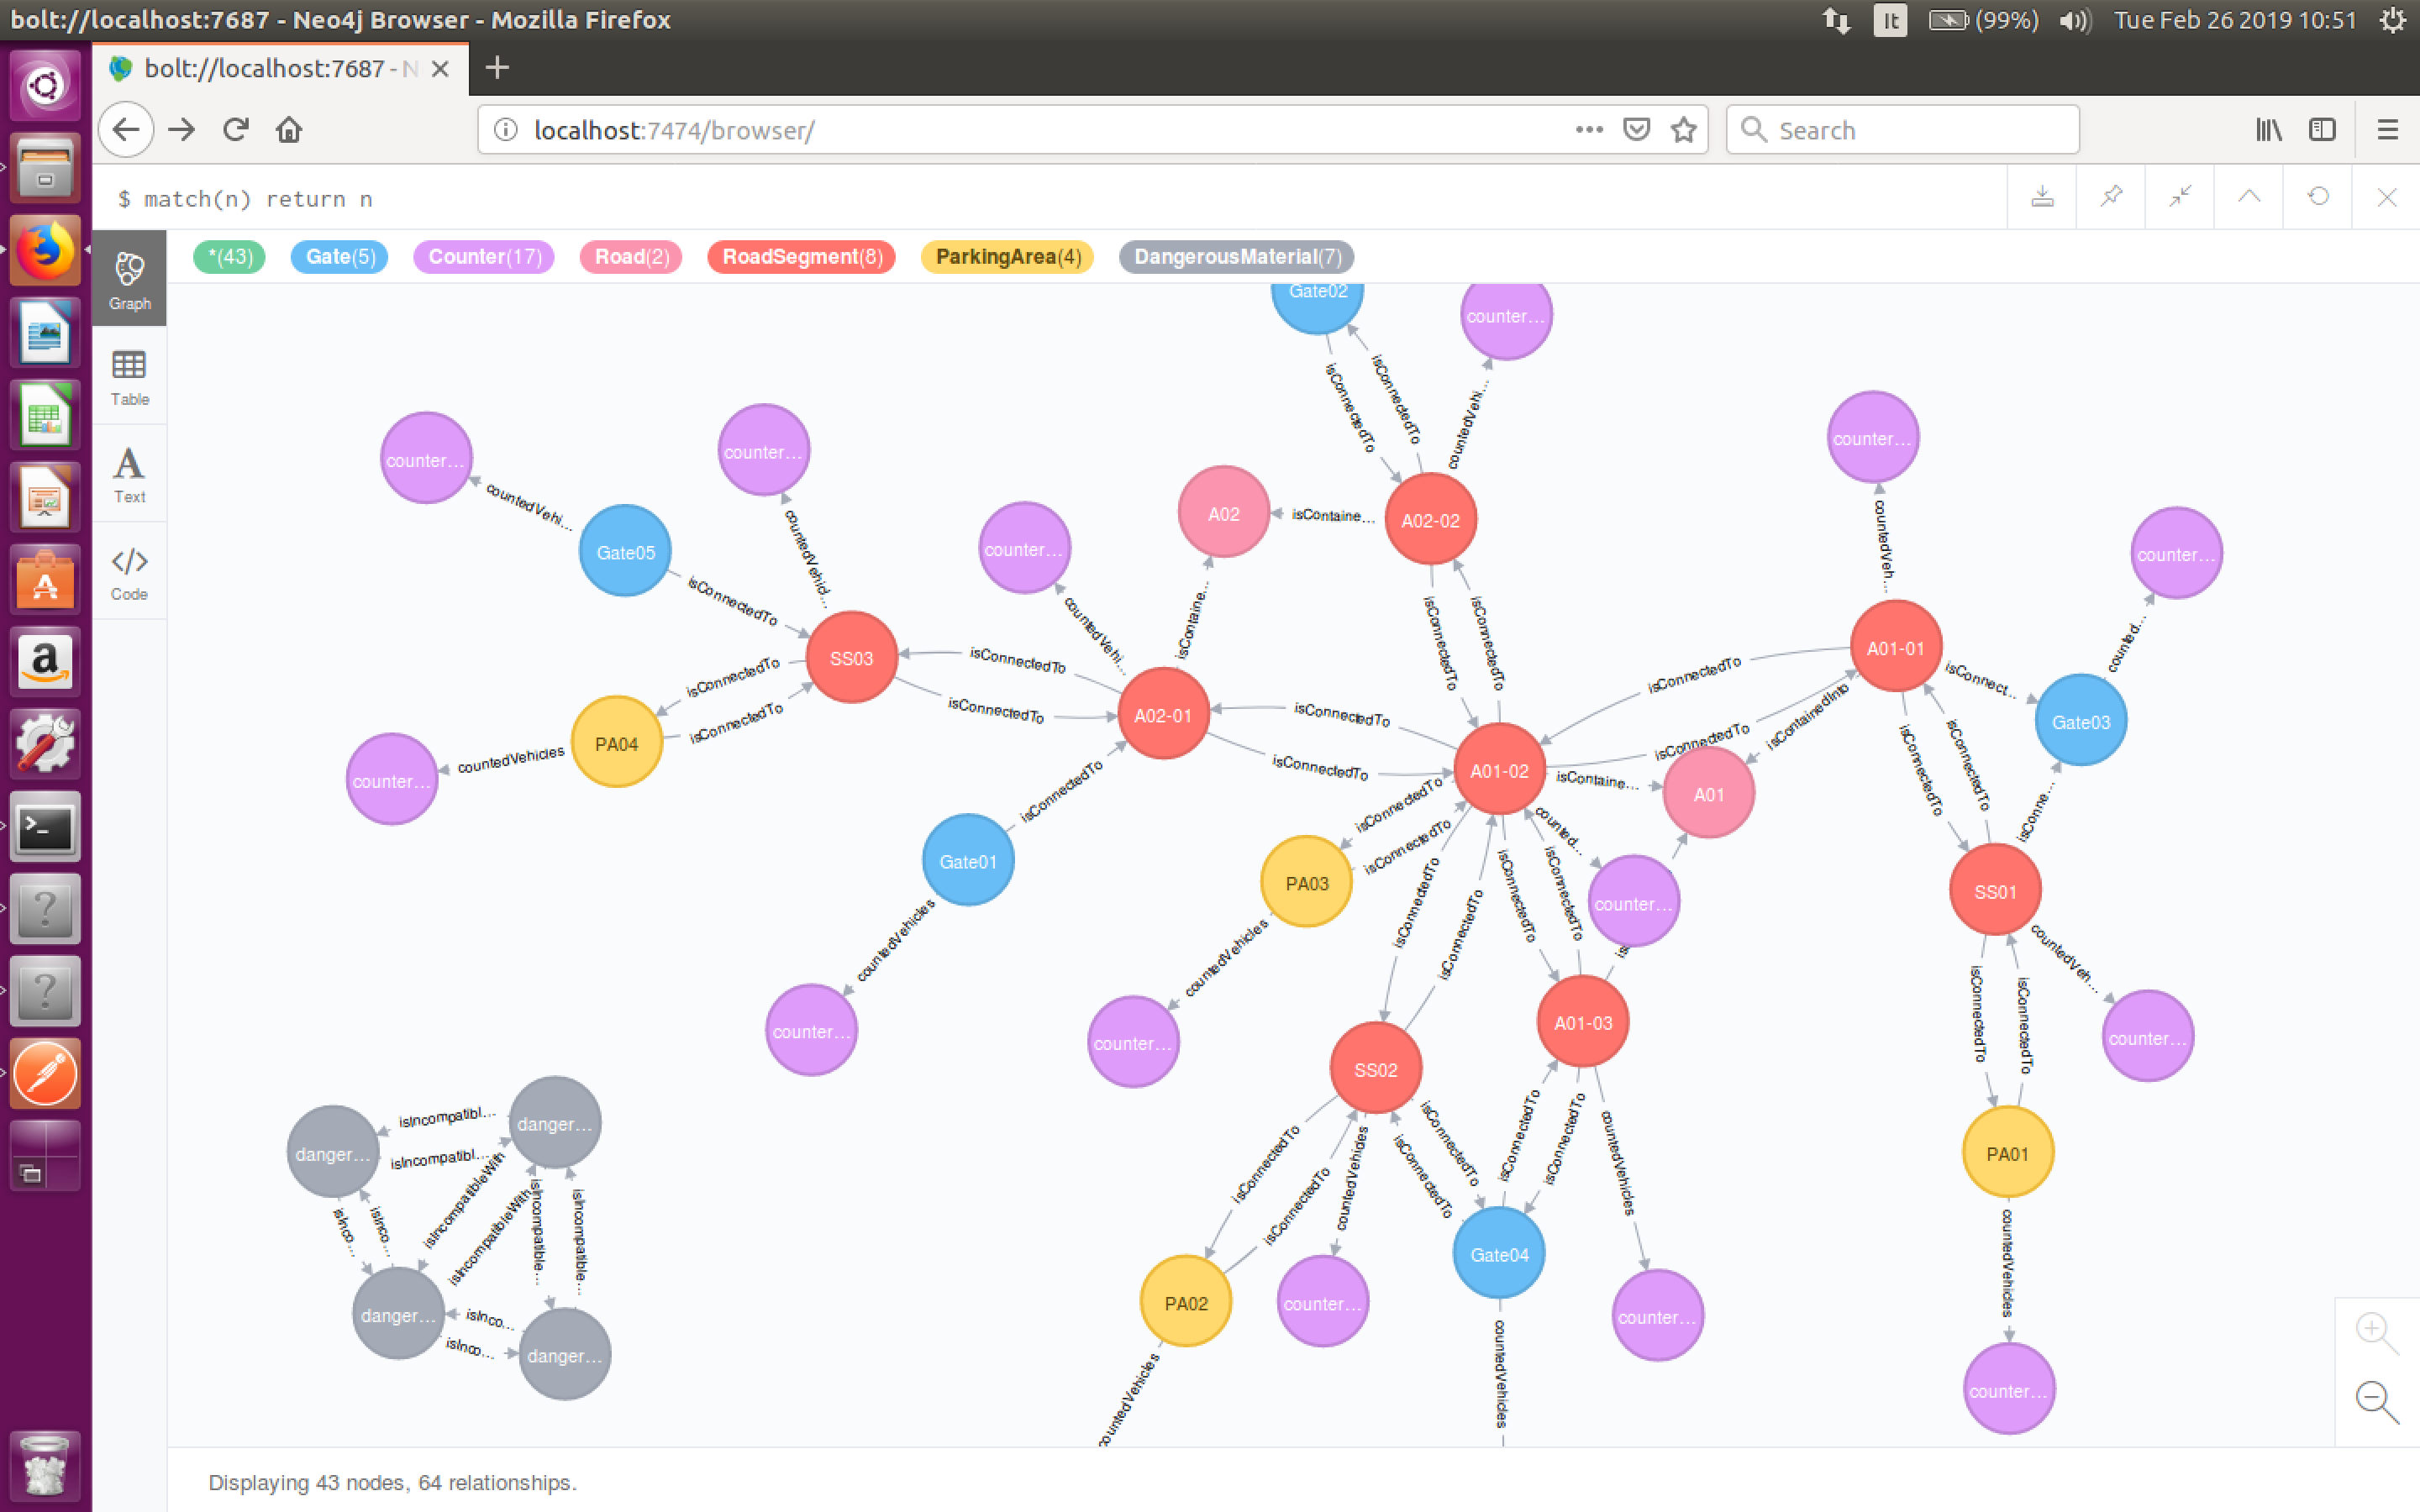
\includegraphics[width=\textwidth]{neo4j_graph.png}
   \caption{Example of graph of the system.}\label{Fig:Neo4jGraph}
\end{figure}
In figure \ref{Fig:Neo4jGraph}, it is represented a possible description of a system where there are present gates, parking area, road segments and road. Other than that, worth of a notice is the presence of some particular nodes:
\begin{itemize}
  \item \textbf{counter} nodes (\textit{purple} nodes in figure \ref{Fig:Neo4jGraph}): this kind of nodes are used to track information about places. There is a counter node for each place and it is responsible of keeping the number of reservations for that place and the number of vehicles that have passed through that place;
  \item \textbf{dangerous material} nodes (\textit{gray} nodes in figure \ref{Fig:Neo4jGraph}): it is present a node, for each dangerous material known by the system. Between these nodes exist relations of incompatibility, in order to allow the system to recognize if a material is incompatible with another.
\end{itemize}

%%%----------------------------------------------------------
\chapter{Client}\label{Chap:Client}
The client is a web application developed in Angular. It is designed to choose and simulate the vehicle journey inside a given map.

\section{Client architecture}
The client is composed by two pages:
\begin{itemize}
	\item Home page: where it is possible to choose the path
	\item Route page: where it is possible to see the route and the next directions to take.
\end{itemize}
The application uses a service to make HTTP requests to the server to retrieve the information needed and another one to share data inside the client.
\newpage

\section{Home page}

In the home page is displayed the actual position of the vehicle in the system, if it has one, as shown in figure \ref{Fig:Position}.

\begin{figure}[!htb]
	\centering
	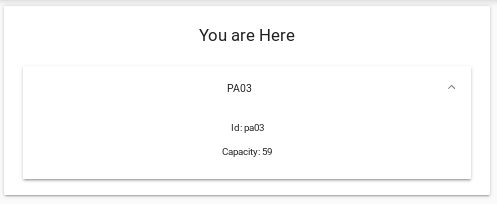
\includegraphics[width=.8\textwidth]{position.png}
	\caption{Actual position in the system.}\label{Fig:Position}
\end{figure}

All info of the places are retrieved using the API of the server \textit{/rns/webapi/rns}, starting point to obtain a map. It is then possible to decide the origin and destination of the vehicle, in order to retrieve an authorization from the server and a path that should be followed, from the list as per figure \ref{Fig:src_dst}.

\begin{figure}[!htb]
	\centering
	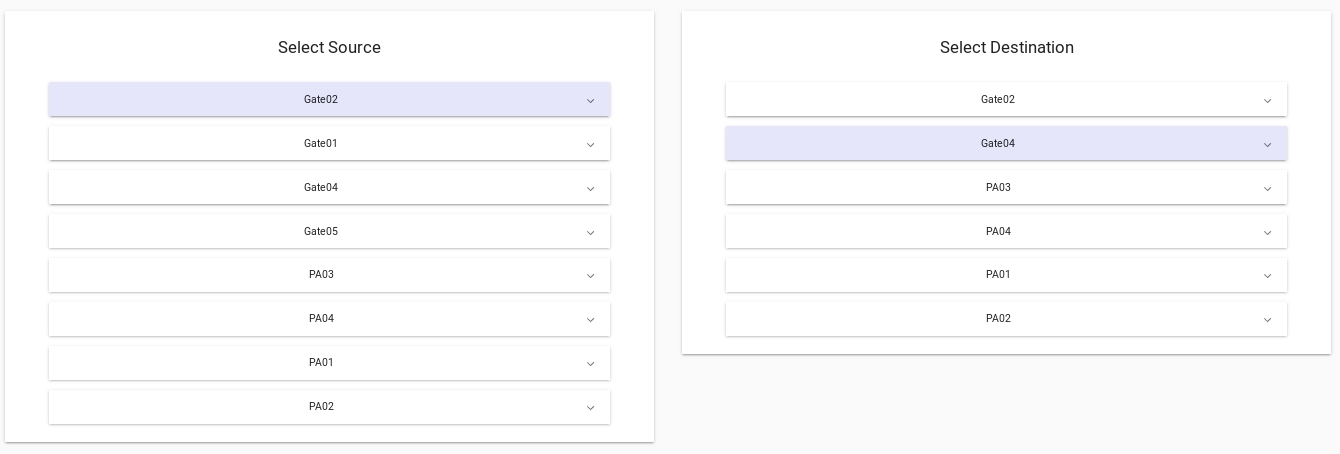
\includegraphics[width=.8\textwidth]{path_src_dst.png}
	\caption{Possible choices of source and destination.}\label{Fig:src_dst}
\end{figure}

\newpage
Also dangerous material are displayed at the end of the page, where it is possible to select only compatible materials.

\begin{figure}[!htb]
	\centering
	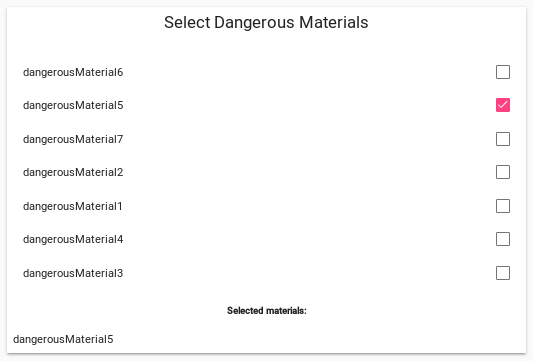
\includegraphics[width=.8\textwidth]{dangerous_mat.png}
	\caption{Possible choices of source and destination.}\label{Fig:dangerous_mat}
\end{figure}

It is then possible to create a POST request using JSON with all the information collected, that are summarized as seen in figure \ref{Fig:path_info}.

\begin{figure}[!htb]
	\centering
	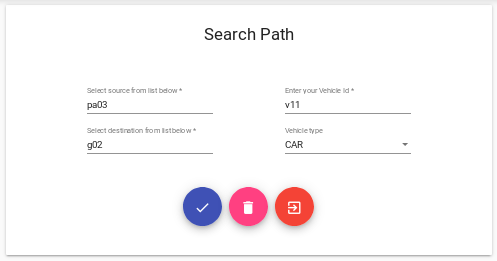
\includegraphics[width=.8\textwidth]{path_info.png}
	\caption{Possible choices of source and destination.}\label{Fig:path_info}
\end{figure}

\newpage
\section{Route page}
The client then redirects to the route page, where it is simulated the journey of the vehicle, by randomly choosing, at every crossroad, the next road to take.
It is the used a PUT request to update the position of the vehicle on the server.
The design was implemented in such way to test the correct behavior of the server in case of error.
The probability to chose a wrong road is constant and defined as 90\%. In this eventuality the server recompute a path and the client is updated.

\begin{figure}[!htb]
	\centering
	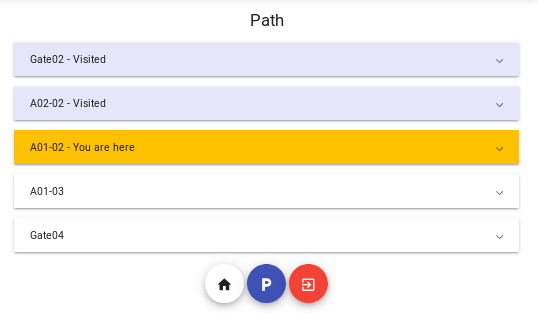
\includegraphics[width=.8\textwidth]{route_page.png}
	\caption{Simulation of the path of the vehicle.}\label{Fig:route}
\end{figure}

%%%----------------------------------------------------------
\chapter{Project setup}\label{Chap:Setup}
In this section will be described the necessary steps to have the application up and running.
\section{Necessary libraries}
The setup of the necessary libraries and framework has been done simmetrically to the one performed in DP2 virtual machine available on the course website. Only difference is the addition of Z3 library for the machine, the setup of it is shown in section \ref{SubSec:Z3Setup}. In figure \ref{Fig:OptFolder} is shown the actual setup used for the machine.
\begin{figure}[!htb]
   \centering
   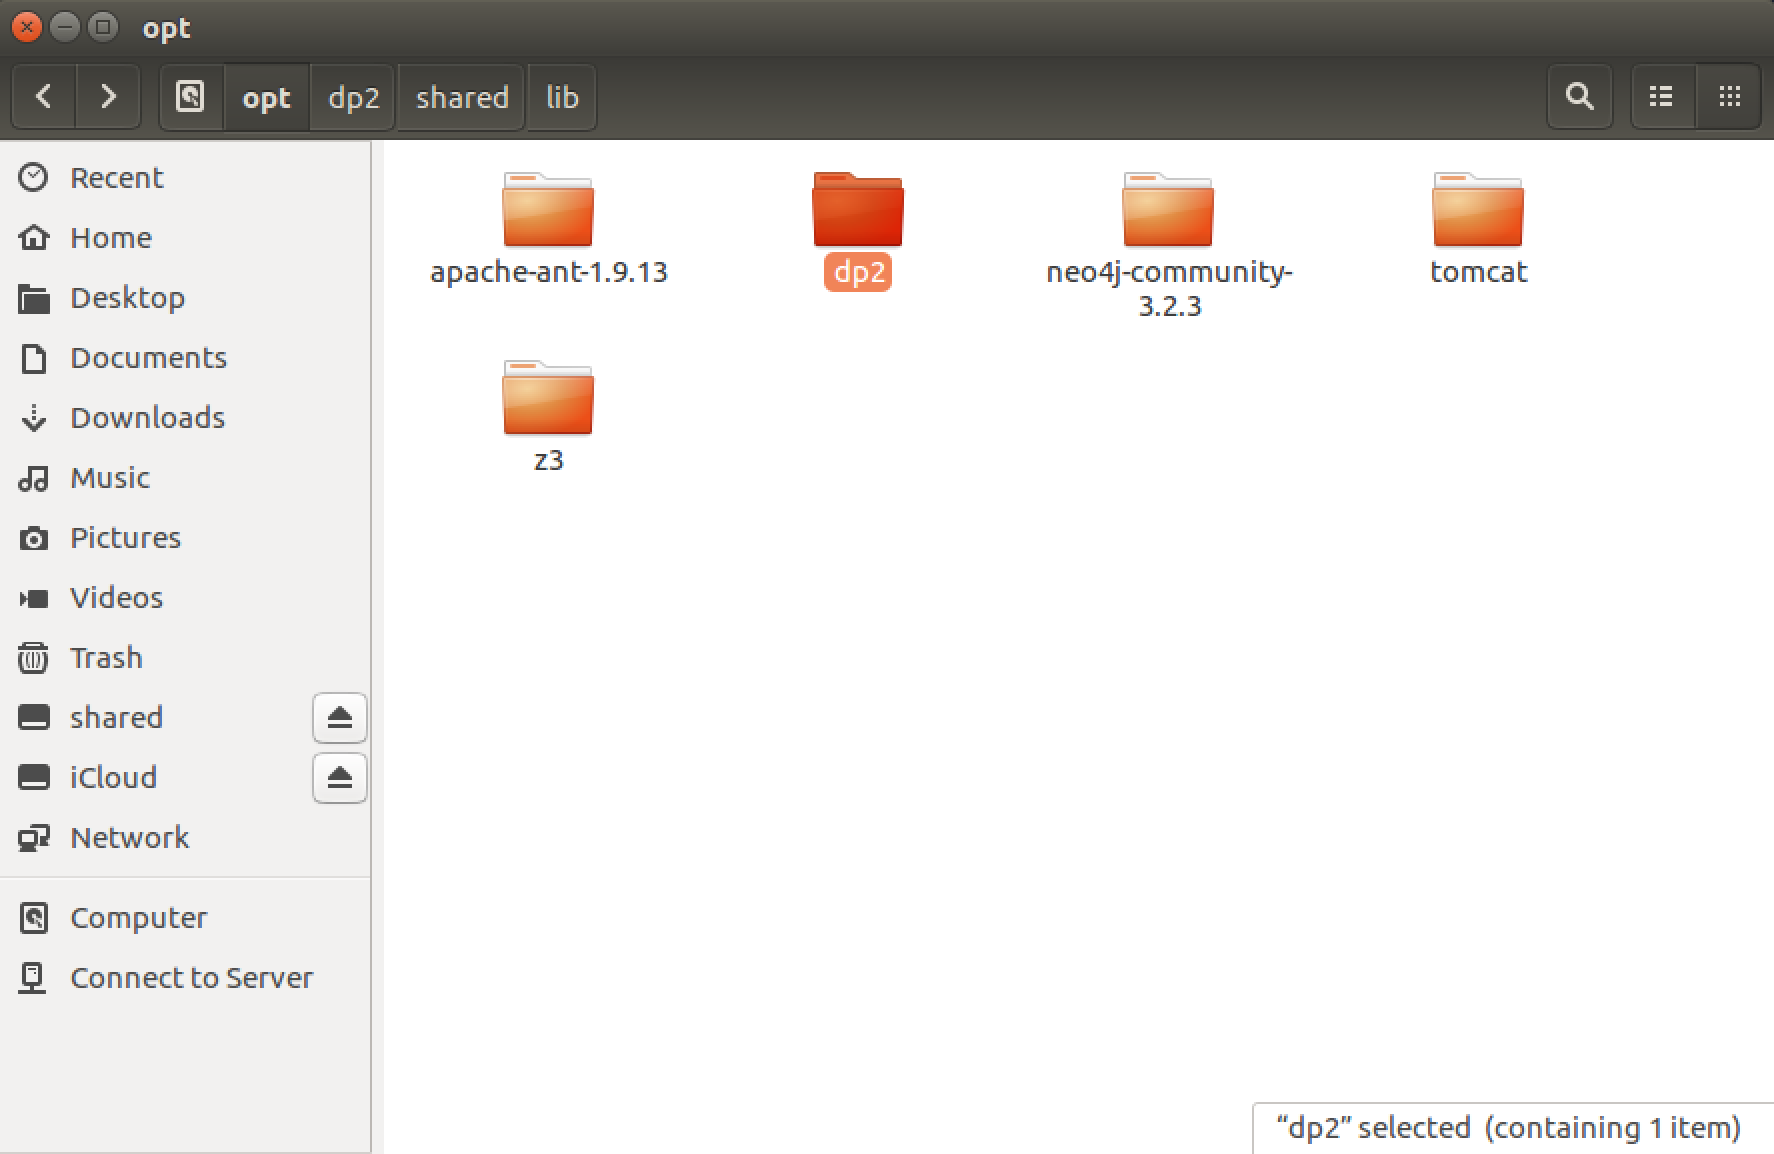
\includegraphics[width=\textwidth]{opt_folder.png}
   \caption{Folder \textit{/opt} of the machine used as development environment.}\label{Fig:OptFolder}
\end{figure}
Additional library like neo4j drivers and junit are provided in the \textit{lib} and \textit{lib-src} folder of the application project. They are already included in classpath during compilation launched through ant scripts. If errors are signaled by Eclipse when opening the project, probably they should be added to build path. After the addition it is suggestable to refresh and clean the project.

\section{Server application and tests}
In order to launch and compile server application, tests and neo4j, a set of ant scripts. In particular:
\begin{itemize}
  \item ant script \textbf{neo4j-build.xml} provides a set of target to launch/stop/restart\&clean neo4j database;
  \item ant script \textbf{build.xml} provides all the target to start/stop tomcat, to deploy the application and to run tests, it relies upon another script to define the operation of such targets, that is \textbf{build-rns.xml}.
\end{itemize}
The targets can be either launched via Eclipse IDE or command line. \\
To setup the server up and running it is necessary to follow these step:
\begin{enumerate}
  \item start Neo4j by using \textbf{start-neo4j} target of \textbf{neo4j-build.xml} script. From command line \textit{ant 'start-neo4j' -f /path/to/neo4j-build.xml};
  \item start Tomcat by calling \textbf{start-tomcat} target of \textbf{build.xml} script. From command line \textit{ant 'start-tomcat' -f /path/to/build.xml};
  \item deploy web service by calling \textbf{redeploy} target of \textbf{build.xml} script. From command line \textit{ant 'redeploy' -f /path/to/build.xml}.
\end{enumerate}
This last command embed in itself the generation of the bindings from XML Schema with JAXB and the compilation of all the necessary classes.\\
In order to launch the tests written for the service it is necessary to use \textbf{rns-tests} target of \textbf{build.xml} script. This target will launch the coompilation of all the classes necessary to the tests and launch them with JUnit.

%%%----------------------------------------------------------
\begin{thebibliography}{1}
\bibitem{tomcat}
  Apache Tomcat website, \texttt{\url{http://tomcat.apache.org/}}
\bibitem{neo4j}
  Neo4j website, \texttt{\url{https://neo4j.com/}}
\bibitem{neo4jcypher}
  Neo4j Drivers documentation, \texttt{\url{https://neo4j.com/docs/driver-manual/1.7/}}
\bibitem{neo4jhttprest}
  Neo4j HTTP REST API documentation, \texttt{\url{https://neo4j.com/docs/http-api/3.5/}}
\bibitem{z3}
  Z3 Prover, \texttt{\url{https://github.com/Z3Prover/z3}}
\bibitem{knapsack}
  Knapsack Problem Wikipedia, \texttt{\url{https://en.wikipedia.org/wiki/Knapsack_problem}}
\bibitem{angular}
Angular, \texttt{\url{https://angular.io/docs}}  
\end{thebibliography}


\end{document}
